%課題研究レジュメテンプレート ver. 1.2

\documentclass[uplatex]{jsarticle}
\usepackage[top=20mm,bottom=20mm,left=20mm,right=20mm]{geometry}
\usepackage[T1]{fontenc}
\usepackage{txfonts}
\usepackage{wrapfig}
\usepackage[expert,deluxe]{otf}
\usepackage[dvipdfmx,hiresbb]{graphicx}
\usepackage[dvipdfmx]{hyperref}
\usepackage{pxjahyper}
\usepackage{secdot}

\makeatletter
  \renewcommand{\section}{%
    \if@slide\clearpage\fi
    \@startsection{section}{1}{\z@}%
    {\Cvs \@plus.5\Cdp \@minus.2\Cdp}% 前アキ
    {.5\Cvs \@plus.3\Cdp}% 後アキ
    %{\normalfont\Large\headfont\raggedright}}
    {\normalfont\raggedright}}

  \renewcommand{\subsection}{\@startsection{subsection}{2}{\z@}%
    {\Cvs \@plus.5\Cdp \@minus.2\Cdp}% 前アキ
    {.5\Cvs \@plus.3\Cdp}% 後アキ
    %{\normalfont\large\headfont}}
    {\normalfont}}

  \renewcommand{\subsubsection}{\@startsection{subsubsection}{3}{\z@}%
    {\Cvs \@plus.5\Cdp \@minus.2\Cdp}%
    {\z@}%
    %{\normalfont\normalsize\headfont}}
    {\normalfont}}
\makeatother
%ここから上を編集する必要はない.





\title{\vspace{-14mm}プロジェクトで発生するリスクのMBTIを用いた事前予測}
\author{PMコース 矢吹研究室 1442085 中村真悟}
\date{}%日付を入れる必要はない.
\pagestyle{empty}%ページ番号は振らない.
\begin{document}
\maketitle


\section{研究の背景}

プロジェクトマネジメントとはヒト・モノ・カネ・資源を管理することである.この中で最もプロジェクトに関わり,かつ対処しにくいのはヒトであると私は考える.

プロジェクトの性質上,そのプロジェクトに合った最適なメンバが選ばれるため,毎回メンバが同じということは保証されない.ならば,プロジェクトマネージャがより早くメンバのことを,人間的特徴を把握することができればより良いマネジメントを行うことに繋がる.

ユングの類型論を発展させたMBTIというものがある.人の考え方を
\begin{itemize}
\item 内向:I・外向:E
\item 感覚:S・直感:N
\item 思考:T・感情:F
\item 判断的態度:J・知覚的態度:P
\end{itemize}
の4指標の組み合わせで16タイプに分類するものである.この技法はキャリアカウンセリングやリーダーシップ開発,チームビルディングなどに使われることが多い\cite{mbti}.

このMBTIを用いて,プロジェクトのメンバの大まかな性格を理解し,メンバの相互作用が原因となって起きる事象を予測したい.
以上のことから本研究ではMBTIを用いて,プロジェクトのリスクに関する事象を予測する方法を研究する.




\section{研究の目的}

本研究の目的は,チームメンバのMBTIの16タイプの相互作用がプロジェクトにどのような影響をもたらしているのかを調べ,MBTIのタイプに基づいてメンバ間で発生しやすいリスクを予測することである.



\section{プロジェクトマネジメントの関連}

本研究は,リスクの予測を目的としているためPMBOKにおけるリスク・マネジメントに該当する.MBTIは自己理解メソッドであり自己成長を促すため,人的資源マネジメントにも関連している.また,MBTIはチームビルディングに用いることができ,メンバ間の円滑なコミュニケーション向上が期待できるため,MBTIはコミュニケーションマネジメントに応用できる.

\section{研究方法}

以下の手順で研究を進める.
\begin{itemize}
\item ソフトウェアコースのPM実験を受講する学生に対し,MBTIの性格検査を行いタイプを調査する
\item その学生に対しアンケートを行い,実際にどのような事象が起きたか調査する
\item アンケートの結果と個人のタイプの組み合わせでどのような関連があるのかを考察する
\end{itemize}


\section{現在の進捗状況}

上記の手順で,PM実験のソフトウェアコースを受講していた学生38人にMBTI診断とアンケート調査を行った.MBTI診断の結果は表\ref{wariai}の通りである.今回診断した学生38人で,16タイプ中13タイプがいた.

表\ref{ke1},\ref{ke2}ははチーム内のMBTIタイプの組み合わせとアンケート結果を集計したものである.メンバとチームの他のメンバとの関係で列,質問の回答を行である.期待度は集計表の合計の結果をもとに算出された値である.この値は「当人とチームの他のメンバのタイプの関係と情報共有が出来ていたかには相関がない」という帰無仮説に基づいた場合の値となる.Z値とは集計表と期待度のずれを計算したものである.このZ値の5%を下回るのであれば帰無仮説は棄却される.

この集計表(表\ref{ke})をχ2乗検定して「当人とチームの他のメンバのタイプの関係と情報共有が出来ていたか」という相関の有無を検討した結果,「内向(I)型:外向(E)型の関係では自分とは違うタイプがいると情報共有しにくい」傾向であることがわかった.
上記と同様に集計表(表\ref{ke2})をχ2乗検定して「当人とチームの他のメンバのタイプの関係と情報共有が出来ていたか」という相関の有無を検討した結果,「規範(J)型:柔軟(P)型との関係では自分とは同じタイプがいると情報共有しにくい」傾向であることがわかった.
\begin{figure}[h]
   \begin{tabular}{c}

      % 1
      \begin{minipage}{0.33\hsize}
        \begin{center}
   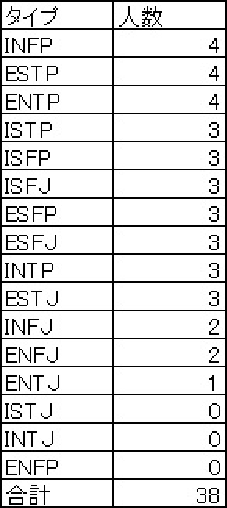
\includegraphics[width=3cm,clip]{wariai.pdf}
  \caption{MBTI結果}
  \label{wariai}
  \end{center}
 \end{minipage}

 \begin{minipage}{0.6\hsize}
   \begin{center}
  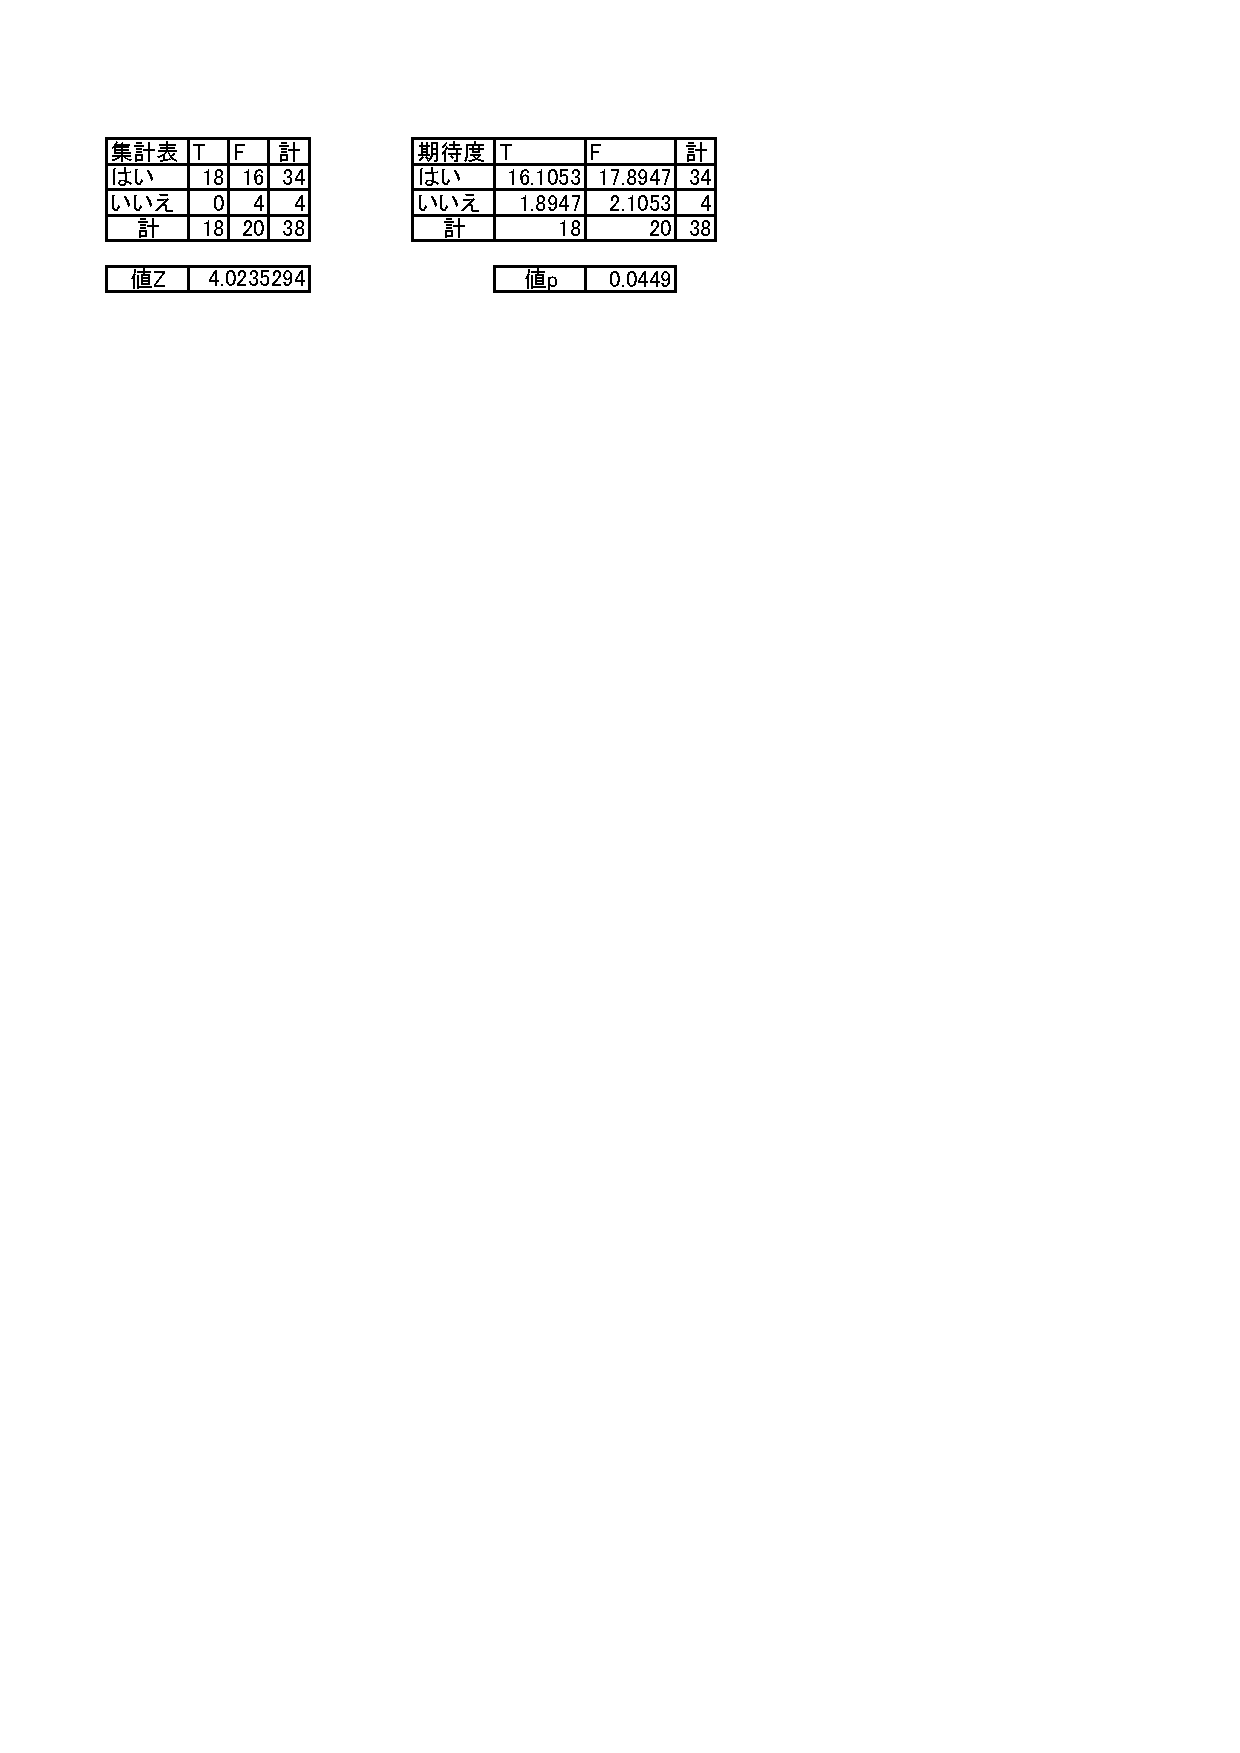
\includegraphics[width=8.2cm,clip]{kekka.pdf}
  \caption{I・Eの関係と情報共有したかの回答結果のクロス集計}
  \label{ke1}
   \end{center}
    \begin{center}  
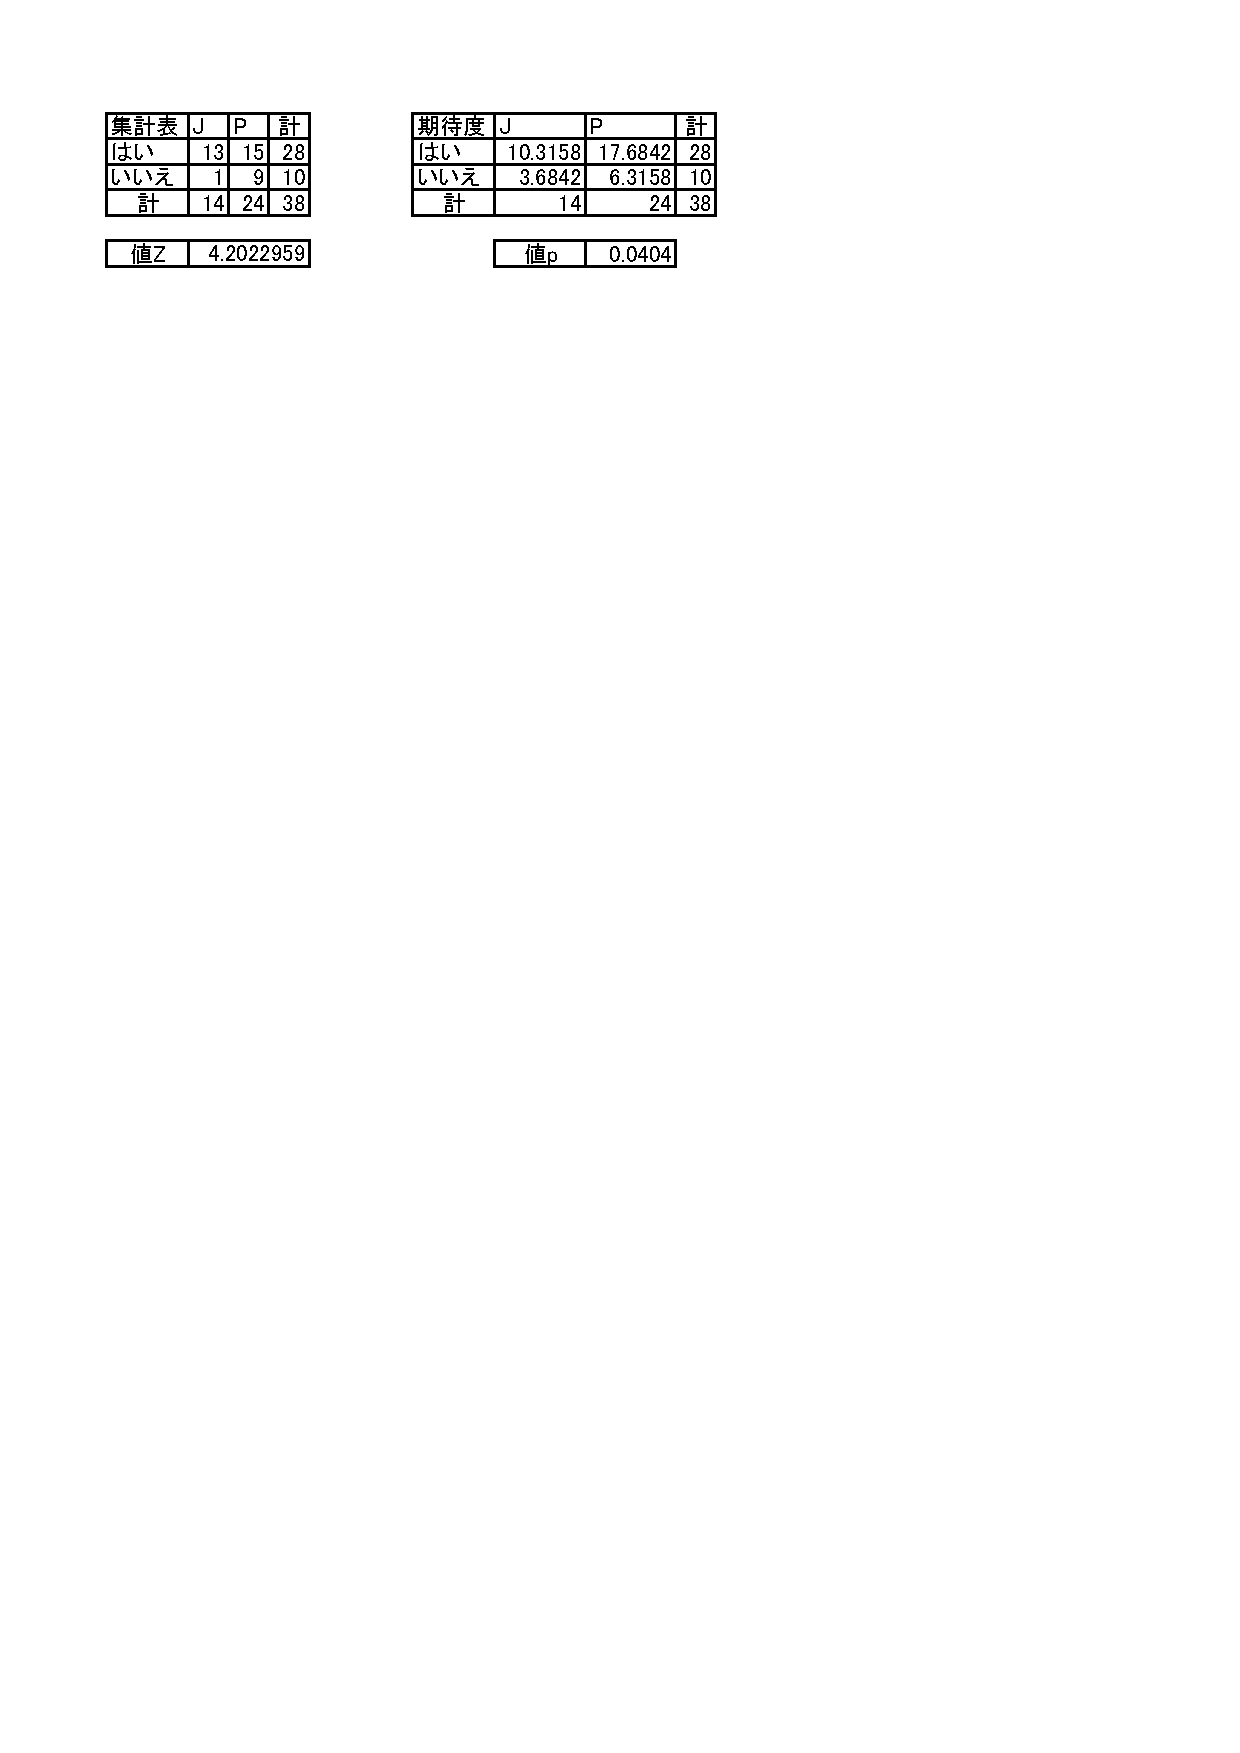
\includegraphics[width=8.2cm,clip]{kekka2.pdf}
  \caption{J・Pの関係と情報共有したかの回答結果のクロス集計}
  \label{ke2}
   \end{center}
 \end{minipage}
\end{tabular}
  \end{figure}


\section{今後の計画}
以下の手順で計画を進める.
\begin{itemize}
\item 今回の結果から相関があったアンケートの項目を掘り下げる
\item PM演習を受講する学生に対し同様の方法でアンケートをPM演習の間3回,発表後1回を行う
\end{itemize}




\nocite{BB19543658}\nocite{110003745117}\nocite{ylab2015}\nocite{katolab2015}
\bibliographystyle{junsrt}
\bibliography{biblio}%「biblio.bib」というファイルが必要.

\end{document}